\documentclass[journal=jpcafh,manuscript=article,layout=onecolumn, 12pt]{achemso}
\usepackage[version=3]{mhchem} % Formula subscripts using \ce{}
\usepackage[T1]{fontenc}       % Use modern font encodings
\usepackage{amsmath}
% NB added command for in line cite
\newcommand{\onlinecite}[1]{\hspace{-1 ex} \nocite{#1}\citenum{#1}} 
%
\author{B.~A.~Laws}
\email{b.laws@unsw.edu.au}
\author{Z.~Levey} 
\author{B.~R.~Lewis}
\author{R.~Mabbs}
\author{S.~T.~Gibson}
\affiliation{Research School of Physics and Engineering, The Australian
	National University, Canberra ACT 2601, Australia}
\title{The H$_2$CCN$^-$ Dipole Bound State and implications for the Diffuse Interstellar Bands}
\abbreviations{PES,PAD,EA,eKE,FWHM,VMI}
\begin{document} 
\begin{abstract} 
	Abstract...
\end{abstract}
\section{Introduction}
Over the past 40 years, photoelectrons spectroscopy has proven to be an effective technique to study the vibrational, rotational, and fine structure of negative ions. Less success has been achieved in the study of electronic transitions, due to the simple fact that the relatively (compared to neutrals) low electron binding energy <~ 3 eV does not leave much `room' for higher states, making anion excited valance states rare. However, if a neutral core has a strong permanent dipole moment > 2 D, it is possible to trap an additional electron in the short-range $1/r^2$ dipole potential. This dipole-bound electronic state behaves similarly to Rydberg states in neutrals, with the valance electron weakly bound ($\sim 100$cm$^{-1}$) in a very diffuse orbital, where the dipole-bound state geometry is similar to that of the neutral core. Due to the short range $1/r^2$ dipole potential, only one or two bound states will be supported, as opposed to the infinite Rydberg series found in neutral molecules where the electron is bound in a long range $1/r$ potential.

Similarly to standard valance excited state spectroscopy, it is possible to excite an anion in the ground state up into it's dipole bound state. As these states are only weakly bound, they will usually undergo subsequent autodetachment down to the neutral. In a photoelectron experiment, this will manifest as resonances in the total photoelectron yield. Therefore, these electronic transitions from the anion up into the DBS may be probed by scanning the detachment wavelength and searching for resonances. Conversely, measuring the kinetic energy of the detached electrons will reveal information about the autodetachment mechanisms. By combining both of these procedures, the entire pathway from anion $\rightarrow$ dipole-bound state $\rightarrow$ neutral + $e^-$ may be mapped out. While the potential of dipole bound state spectroscopy has been long known, it has only recently started to be explored in detail experimentally. Furthermore, the current autodetachment theory and proposed selection rules that is employed in these studies has yet to be tested against a high resolution experimental study of both vibrational and rotational DBS autodetachment. 

The cyanomethylide anion H$_2$CCN$^-$ is a valuable prototype for studying the spectroscopy of dipole bound states. With a permanent dipole moment of 3.6 D, H$_2$CCN$^-$ is known to support dipole-bound states, while the ground state anion has been well studied as a benchmark system for ion thermochemistry studies. In fact many of the recent DBS studies have focussed on this molecule, as the state can undergo both rotational autodetachment near threshold, and vibrational detachment above threshold, with non-zero electron kinetic energies. Because of the variety of different detachment pathways available, H$_2$CCN$^-$ was employed as a test case for a recently published summary of autodetachment theory and proposed selection rules. This research is also motivated by potential astrochemical implications, as the transition from the electronic ground state to the DBS of H$_2$CCN$^-$ has been put forward as a plausible carrier of the 8037\AA~ diffuse interstellar band. This suggestion has lead to further discussion around the suitability of other anion DBS transitions as potential DIB carriers. 
  
In this work, the spectroscopy of dipole-bound states is examined in detail, by studying H$_2$CCN$^-$ using a high-resolution photoelectron imaging (HR-PEI) spectrometer. Photoelectron measurements are examined at a large range of wavelengths (355-805~nm) to explore different detachment mechanisms above, near, and below threshold. Fixed wavelength velocity-map image experiments are combined with wavelength scanning electron yield measurements to build a complete model of dipole bound state spectroscopy from anion to neutral. This model is then used to explore the possibility that H$_2$CCN$^-$ is responsible for the 8037\AA~ diffuse interstellar band.

\section{Results and Discussion}
Typically photodetachment from a negative ion proceeds via a non-resonant, direct electric dipole transition, form a bound state orbital to a continuum state. However, if an anion can support a dipole-bound state then it is also possible to detach an electron via a resonantly-enhanced one-photon process, involving a non-adiabatic energy transfer that my be mediated by either vibrational or rotational motion. To build a complete model of DBS spectroscopy, H$_2$CNN$^-$ photodetachment was examined at 130 wavelengths, to probe the transition from the anion ground state up into the dipole-bound state, as well as the corresponding direct detachment, vibrational autodetachment, and rotational autodetachment mechanisms.

\subsection{Non-resonant direct photodetachment}
Cyanomethylide ions were produced in a pulsed-jet discharge of a 1:1 gas mixture of C$_2$H$_4$ and N$_2$O, and subsequently mass isolated via time of flight. An illustrative VMI of ~ 3 million photoelectrons collected from 532.1~nm (2.33~eV) non-resonant H$_2$CCN$^-$ photodetachment is shown in Fig.~\ref{fig:532}. The electrons are distributed radially according to their speed, with fast electrons at the detector edge and slow electrons at the image centre. Each dominate ring may be assigned to a vibrational progression for the electronic transition between ground electronic states of the anion and neutral H$_2$CCN($\tilde{X}^2B_1$) + $e^-$ $\leftarrow$ H$_2$CCN$^-$ ($\tilde{X}^1A_1$) + $hv$. The laser polarisation is aligned vertically, with the electrons preferentially distributed around the hemisphere of the image, indicative of a negative anisotropy parameter.

\begin{figure}
	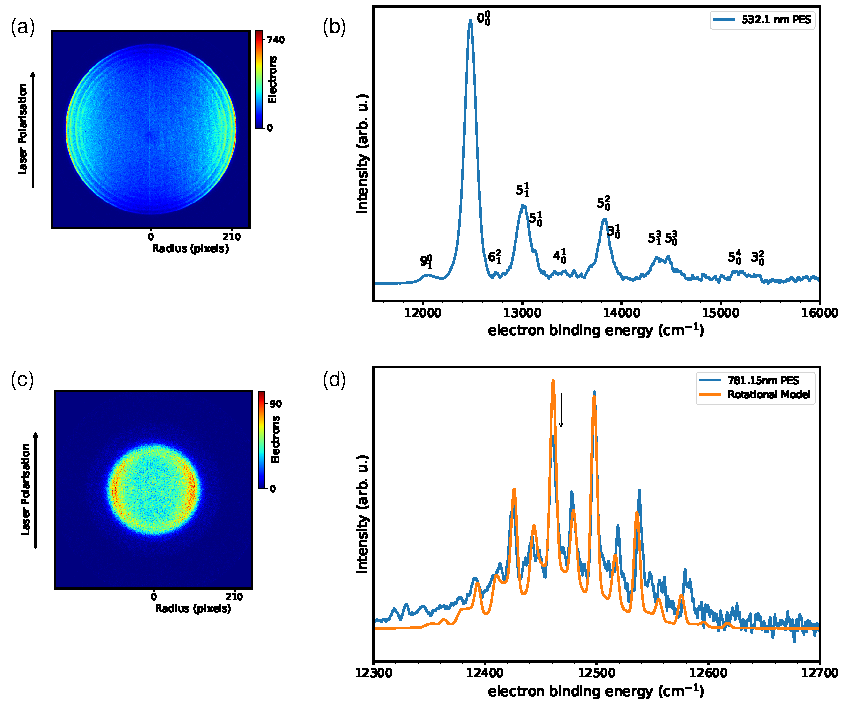
\includegraphics[width=0.5\textwidth]{figures/Fig1}
	\caption{Shine - 532nm PES}
	\label{fig:532}
\end{figure}

The corresponding photoelectron spectrum, extracted via an inverse Abel transformation from the VMI in Fig.~\ref{fig:532}, is shown in Fig.~\ref{fig:532-b}. The H$_2$CCN$^-$ anion has a slightly non-planar $C_s$ geometry, while the ground state of neutral H$_2$CCN is planar, with $C_{2v}$ symmetry. The potential along the anion $v_5 (b_1)$ umbrella coordinate is a shallow double well, with predictions for the inversion barrier ranging from $\sim~100$cm$^{-1}$ to $\sim~150$cm$^{-1}$. At our jet cooled temperature of $\sim150~$K anions produced will usually be predominantly in their vibrational ground state. However here, due to the small inversion splitting, the $5_1$ hot band will be substantially populated. Consequently, the vibrational structure resolved in Fig.~\ref{fig:532-b} may be assigned to two main progressions $5_0^{2n}$ and $5_1^{2n+1}$, offset from each other by $\sim130~$cm$^{-1}$. Note that transitions to the $C_{2v}$ neutral involving an even quanta of $(b_1)$ symmetry vibration (including $v_5$) are forbidden. 

\subsubsection{Rotational Structure}
The energy resolution attainable with velocity map imaging is proportional to the kinetic energy of the imaged particle, i.e. $\Delta\epsilon\propto\epsilon$. Therefore higher resolution spectra may be obtained at longer wavelengths, closer to threshold. A VMI of H$_2$CCN$^-$ non-resonant photodetachment at 781.15~nm, along with the corresponding photoelectron spectrum are shown in Fig.~\ref{fig:781}. At 781.15~nm only the ground vibrational state of the neutral is accessible, however the slower electrons allow for rotational transitions to be resolved. 

\begin{figure}
	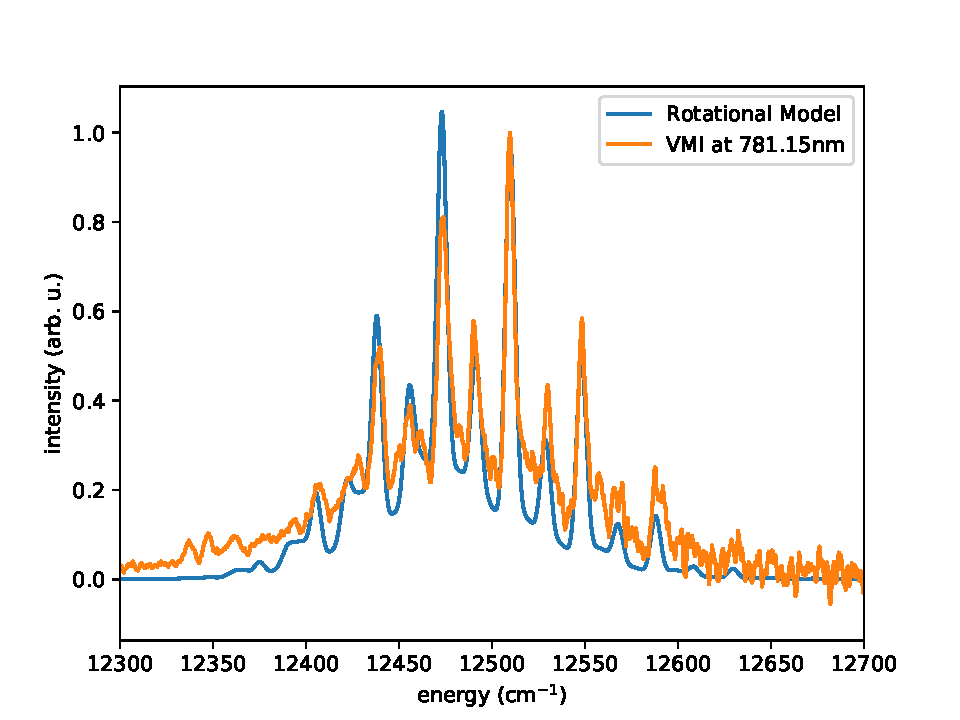
\includegraphics[width=0.5\textwidth]{figures/781rot.pdf}
	\caption{Rotation- 781nm PES}
	\label{fig:781}
\end{figure}

While the cyanomethylide anion is slightly non-planar, it may be treated as having a quasi-planar $C_{2v}$ geometry. Similarly, while both the neutral and anion are strictly asymmetric tops with 3 distinct rotational constants, as A $>>$ B $\approx$ C they can be viewed as near prolate tops. As the molecule has two identical Hydrogen nuclei, the total eigenfunction must be either symmetric or antisymmetric  with respect to a 180$^{\circ}$ rotation around the symmetry (B) axis. Due to the nuclear spin of I(H) = $\frac{1}{2}$, levels that are antisymmetric under this rotation will have a 3:1 weighting compared to symmetric levels. Furthermore, for a planar $C_{2v}$ asymmetric top molecule, the symmetry of consecutive rotational levels a distinct pattern. For both even and odd J, the lowest $\tau_{-J}$ level of each band will by symmetric, followed by two anti-symmetric levels, followed by two symmetric levels, and so on. In the near prolate top limit this becomes $K_{\text{odd}} : K_{\text{even}} = 3:1$. The rotational energy of each level may then be calculated from Eq.~(\ref{eq:rot}),
\begin{equation}
	E(J,K)_{A,B} = BJ(J+1)+(A-B)K^2.
	\label{eq:rot}
\end{equation}

After applying the relevant dipole transition selections rules for a perpendicular transition, $\Delta J = 0,\pm 1$ and $\Delta K = \pm1$, the relative intensity of each allowed transition may be determined from the statistical weights and Boltzmann, Frank-Condon, and H\"{o}nl-London factors. The resulting rotational model was fitted to the experimental photodetachment data at 781.15~nm, as shown in Fig.~\ref{fig:781}. From this an anion rotational temperature of T = 150(x)~K and a FWHM = 6(x)~cm$^{-1}$ were obtained, giving a value for the H$_2$CCN$^-$ electron affinity of EA = xxxx~cm$^{-1}$.

\subsection{Resonant vibrational autodetachment}
While direct photodetachment cross sections vary smoothly (as demonstrated by the Wigner threshold law at low electron kinetic energies), autodetachment introduces sharp resonances, where the electronic ground state of the anion may be excited up into the dipole bound state. After excitation the weakly bound electron may be expelled via a non-adiabatic energy transfer. In the case of vibrational autodetachment, the energy of the DBS excited nuclear vibration is redistributed to the kinetic energy of the departing electron, and the electronic + nuclear energy of the final neutral state,
\begin{equation}
	\text{A}^-(\epsilon_{\text{el}}''+\epsilon_{\text{vib}}'') + hv \rightarrow \text{DBS}^-(\epsilon_{\text{el}}+\epsilon_{\text{vib}}) \rightarrow \text{A}(\epsilon_{\text{el}}'+\epsilon_{\text{vib}}') + e^-.
	\label{eq:energy}
\end{equation}

To explore these vibrational resonances, velocity map images of H$_2$CCN$^-$ were measured at 120 different wavelengths between 600 and 800~nm. Each image consists of $\sim$ 1 million photoelectrons from xxx laser shots, to ensure high resolution is maintained in the electron kinetic energy domain. The resulting photoelectron spectra are presented in Fig.~\ref{fig:PESall}. Each spectrum was normalized with respect to the non-resonant photoelectron spectrum at 532.1~nm (Fig.~\ref{fig:532}) with intensities interpolated between measurements in the y direction, so that any intensity in the 2D plot Fig.~\ref{fig:PESall} represents an autodetachment resonance. The intensity distribution vs wavelength (y-axis) reveals the absorption pathways from the anion ground state up into DBS, while the intensity vs electron binding energy (x-axis) provides information about the autodetachment pathways.

\begin{figure}
	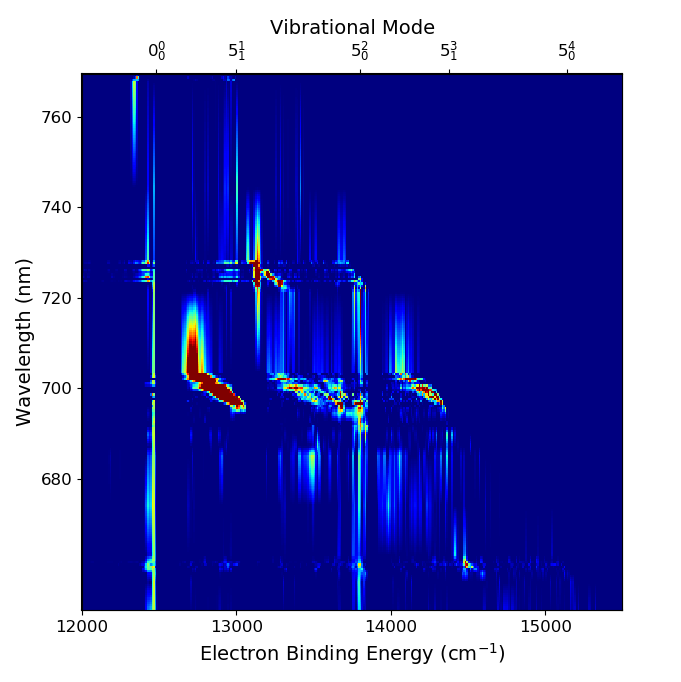
\includegraphics[width=0.5\textwidth]{figures/2DJuly21}
	\caption{2Dplot}
	\label{fig:PESall}
\end{figure}

Figure~\ref{fig:PESall} reveals a range of autodetachment resonances, with many occurring at non-zero electron kinetic energies, well above threshold. Notably, while most resonances appear at a constant binding energy, some of the observed resonances appear to walk with the photon energy. Each individual resonance may be examined in detail, mapping out the entire pathway from anion $\rightarrow$ DBS $\rightarrow$ neutral, to test the current theory of DBS spectroscopy and vibrational autodetachment. As an example, a selection of photoelectron spectra around 661~nm are shown in Fig.~\ref{fig:661} alongside a depiction of the relavant H$_2$CCN$^-$ potential energy surfaces. Electron energies are plotted in Binding Energy.

\begin{figure}
	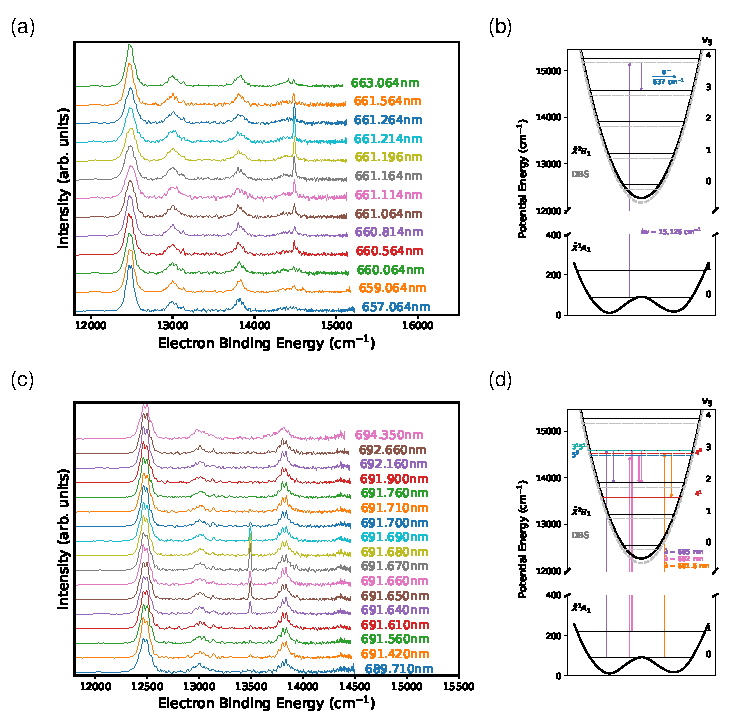
\includegraphics[width=0.5\textwidth]{figures/Fig3}
	\caption{resonance at 661}
	\label{fig:661}
\end{figure}

A clear resonance can be seen in Fig.~\ref{fig:661} at a wavelength of $\sim661.2~$nm and binding energy of $\sim14500~\text{cm}^{-1}$. A plot of the integrated intensity between $14,450-14,650$~cm$^{-1}$ vs photon energy for all of the collected spectra in this region is shown in Fig.~\ref{fig:661}. From this, an absorption energy of E$_{\text{abs}}=15,126.8(2)~\text{cm}^{-1}$ was obtained, representing the transition energy from the anion ground state up into an excited vibrational state of the DBS. Similarly, the resonance position in the electron kinetic energy domain reveals a transition energy from the DBS to the neutral of E$_{\text{detach}}=637.0(1)~\text{cm}^{-1}$. By comparing these values to the potential energy surfaces in Fig.~\ref{fig:661}, this resonance may be assigned to the transitions
\begin{align*}
	\text{A}^-(0^0) +hv \rightarrow \text{DBS}^-(5^4) \rightarrow \text{N}(5^3) + e^-,
\end{align*}
representing the entire pathway from anion to neutral. This vibrational autodetachment mechanism follows both the normal mode constraint ($v_5\rightarrow v_5$) and the $\Delta v = -1$ propensity rule.

\subsubsection{Autodetaching mechanisms}
Not all of the resonances found in this study appear to follow the same behaviour. Some autodetaching resonances appear very sharp, in both the electron and photon energy domains, whereas others appear to be much broader. This is demonstrated by the selection of photoelectron spectra presented in Fig.~\ref{fig:691}. 

\begin{figure}
	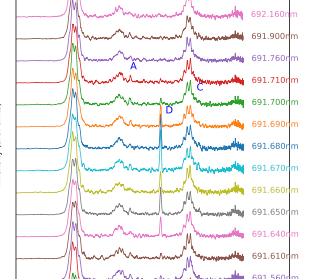
\includegraphics[width=0.5\textwidth]{scripts/691}
	\caption{resonance at 691}
	\label{fig:691}
\end{figure}

At wavelengths of $\sim 691.6$nm, a sharp resonance is observed at $\sim13,500~$cm$^{-1}$ that may be assigned to the transitions
\begin{align*}
	\text{A}^-(0^0) +hv \rightarrow \text{DBS}^-(4^2) \rightarrow \text{N}(4^1) + e^-.
\end{align*}
As the vibrational mode $v_4$ is not active in the non-resonant direct detachment spectrum (Fig.~\ref{fig:532}), this resonance provides a way to experimentally determine the anion frequency $\omega_4 = xxx~$cm$^{-1}$. In Fig.~\ref{fig:691} there is also a second resonance at $\sim13,750~$cm$^{-1}$. However, unlike resonance C, resonance D appears very broad, with the entire rotational band appearing to be enhanced. Furthermore the resonance is present over a larger range of photon energies, $\sim 2~$nm as opposed to $\sim 0.1~$nm. Due to the close lying nature of the $5^3$ and $3^15^1$ vibrational levels in the DBS (only separated by $\sim 150~$cm$^{-1}$ ), multiple detachment pathways may be attributing to this resonance, which may contribute to the broad behaviour,
\begin{align*}
	\text{A}^-(0^0) +hv &\rightarrow \text{DBS}^-(3^15^1) \rightarrow \text{N}(5^2) + e^-,\\
	\text{A}^-(0^0) +hv &\rightarrow \text{DBS}^-(5^3) \rightarrow \text{N}(5^2) + e^-,\\
	\text{A}^-(5^1) +hv &\rightarrow \text{DBS}^-(3^15^1) \rightarrow \text{N}(5^2) + e^-.
\end{align*}
These pathways involve energy being transferred between the CH$_2$ umbrella mode $v_5$ and the CH$_2$ scissors mode $v_3$.

Another anomaly observed in some resonances is highlighted in Fig.~\ref{fig:723}. At $\sim 723~$nm two clear resonances are observed at 13,600 and 13,700~cm$^{-1}$ respectively. They may be assigned to the transitions up into the $3^1$ band of the DBS, detaching to the $6^2$ and $9^2$ bands of the neutral. However as the wavelength increases, while resonance K remains at a constant electron binding energy, peak J appears to 'walk' towards lower binding energies (and towards peak K). This behaviour continues until $\sim$ 726 nm, where both resonances are on top of each other.  As the wavelength increases, the anion goes from being excited into the $3^1$ band of the DBS to the overlapping $5^2$ band. Consequently, as the $5^2$ character of the DBS increases, detachment to the $5^1$ level in the neutral becomes favoured. This highlights how non-adiabatic energy transfers can still occur between different vibrational coordinates, where levels are close in energy. However if it is possible to autodetach via a transition that follows the propensity rules, this pathway will likely be favoured.

\begin{figure}
	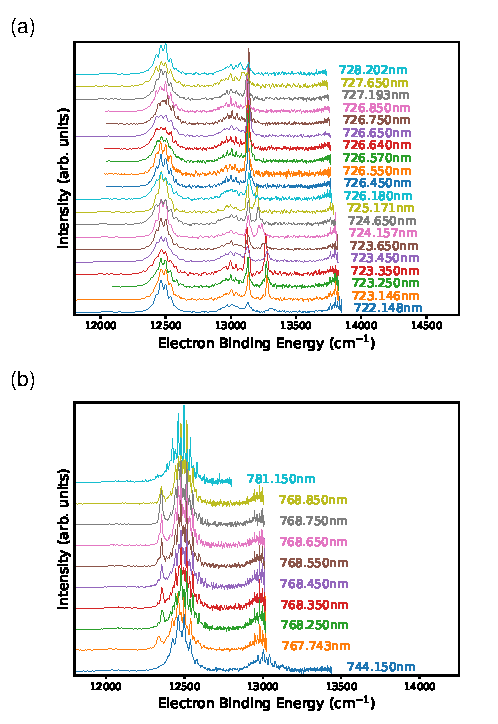
\includegraphics[width=0.5\textwidth]{figures/Fig4}
	\caption{resonance at 723-726}
	\label{fig:723}
\end{figure}

\subsubsection{Inversion splitting in H$_2$CCN$^-$}
Vibrational autodetachment resonances were also observed on the low binding energy side of the origin, below threshold, as shown in Fig.~\ref{fig:768}. A sharp resonance (L) may be seen in photoelectron spectra $\sim 768~$nm at a binding energy of $\sim 12,350~$cm$^{-1}$ - about 100~cm$^{-1}$ lower than the origin at 12,468~cm$^{-1}$. This may be assigned to the $5_1$ hot band origin transition of the anion, 
\begin{align*}
	\text{A}^-(5^1) +hv \rightarrow \text{DBS}^-(5^1) \rightarrow \text{N}(0^0) + e^-.
\end{align*}
Therefore, the difference in energy between resonance L and the origin provides a direct measurement of the inversion splitting $\omega_5$ in the anion. Previously, this value could only be measured by comparing the offset between the $5^{2n}_0$ and $5^{2n+1}_1$ progressions in the non-resonant photoelectron spectrum (Fig.~\ref{fig:532}). This relied on estimates of the rotational band head within each unresolved vibrational transition. However as the rotational band profile is resolved in Fig.~\ref{fig:768}, the true positions of the resonance and the band origin can both be determined, providing an accurate value for the inversion splitting of $\omega_5 = 113(x)~$cm$^{-1}$.

\begin{figure}
	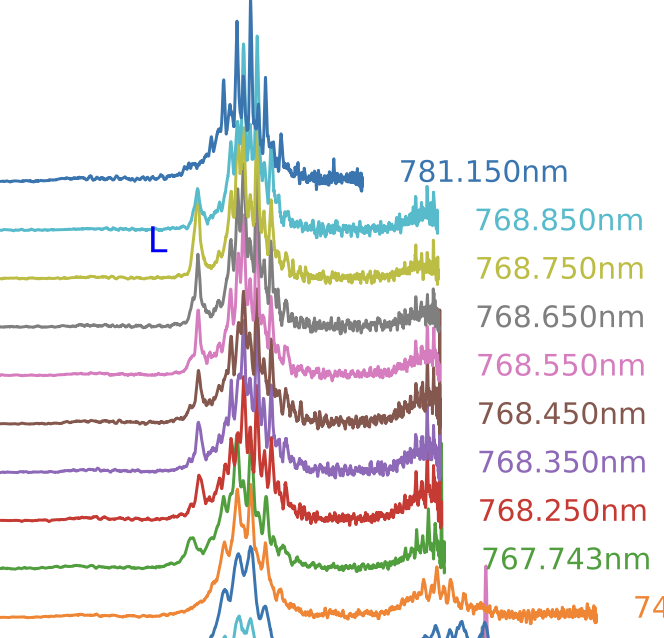
\includegraphics[width=0.5\textwidth]{scripts/768}
	\caption{resonance at 768}
	\label{fig:768}
\end{figure}

In total, XXX vibrational autodetachment resonances were observed within the wavelength range 600-800~nm. The position and possible assignments for each resonance are presented in Table~\ref{tab:peaks}. A wide variety of resonances were found, some which do not follow the expected propensity and normal mode restrictions, some which are assigned to non-active vibrational transitions, and some which can not be readily assigned to any normal-mode transition in the DBS.

\subsection{Resonant rotational autodetachment}
By moving to longer wavelengths, so that only the ground vibrational level of the DBS is energetically accessible, all vibrational autodetachment pathways may be turned off. Therefore, any resonances in the photoelectron spectrum may be assigned to rotational autodetachment, where the excited nuclear rotational energy is non-adiabatically transferred into the kinetic energy of the departing electron, and the electronic + nuclear energy of the final neutral state,
\begin{equation}
	\text{A}^-(\epsilon_{\text{el}}''+\epsilon_{\text{rot}}'') + hv \rightarrow \text{DBS}^-(\epsilon_{\text{el}}+\epsilon_{\text{rot}}) \rightarrow \text{A}(\epsilon_{\text{el}}'+\epsilon_{\text{rot}}') + e^-.
	\label{eq:rot-energy}
\end{equation}
To examine rotational autodetachment of H$_2$CCN$^-$ a velocity mapped image was acquired at one of these resonances, very close to threshold at $\lambda = 801.567~$nm, with the corresponding photoelectron spectrum presented in Fig.~\ref{fig:801}. To assign the observed rotational structure, the entire pathway from anion $\rightarrow$ DBS $\rightarrow$ neutral needs to be modelled. The first step, absorption up into the DBS, follows the same rotational selection rules that were determined for non-resonant direct detachment (Fig.~\ref{fig:768}). Namely, for a perpendicular transition of a prolate symmetric top $\Delta K = \pm 1$ and $\Delta J = 0,\pm1$. At our resonant photon energy $hv = 12475~$cm$^{-1}$, this corresponds to an excitation from the $K''=2$ level of the anion up into the $K=3$ level of the DBS.

\begin{figure}
	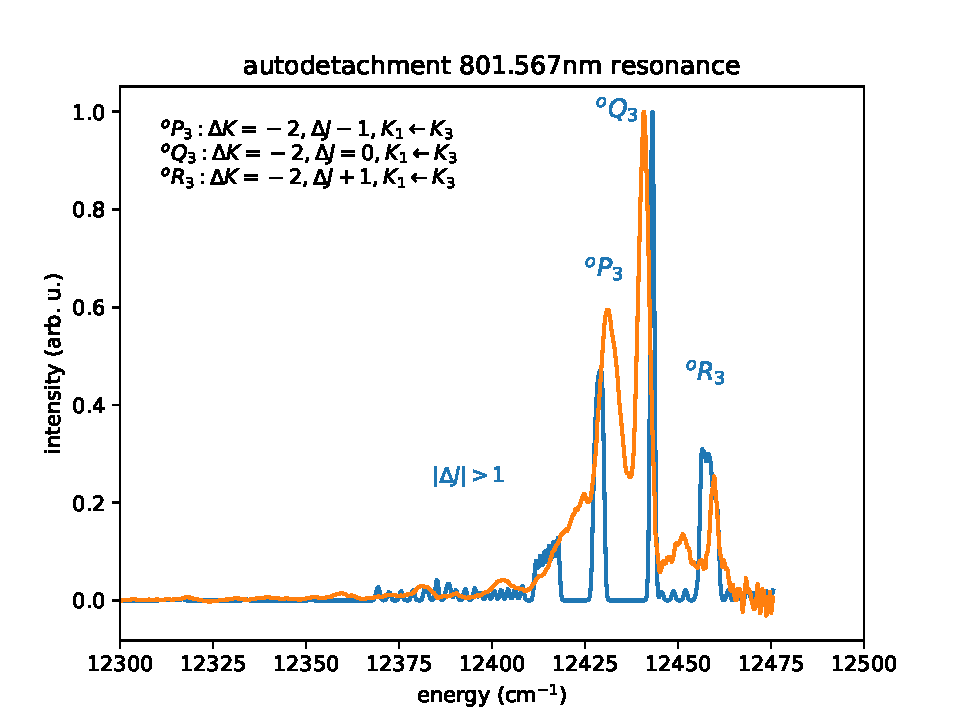
\includegraphics[width=0.5\textwidth]{scripts/801}
	\caption{resonance at 801}
	\label{fig:801}
\end{figure}

However it is the kinetic energy of the autodetached electrons from the second step (DBS $\rightarrow$ neutral) that is measured in a photoelectron experiment. Due to the identical Hydrogen atoms on each side of the $C_{2v}$ axis, the change in $K$ must be even, i.e $\Delta K = 0, \pm2, \pm4, \pm6,... $. Unlike direct detachment, the change in total angular momentum $J$ may be greater than 1, however pathways with the minimum possible change in $J$ will be favoured. It is also important to note that only rotational levels above threshold will autodetach and be observed in our experiment. Therefore the coldest few rotational levels, with E(J,K) < DBS binding energy, will be missing from the experimental spectrum. By combining these selection rules with the rotational model for the first step, it is possible to model the entire pathway from anion $\rightarrow$ DBS $\rightarrow$ neutral. 

The resulting model is shown fitted to the experimental spectrum at 801.567~nm in Fig.~\ref{fig:801}. An illustrative energy level diagram (for J = 20) is also shown, to highlight the dominant autodetaching pathways responsible for this resonance. The 3 dominant peaks in the photoelectron spectrum may be assigned to the P, Q, and R branches ($\Delta J = -1, 0 ,+1$) of the $\Delta K = -2$ autodetachment transition. The complete pathway from anion to neutral is then given by $A^-(K''=2)\rightarrow DBS^-(K=3) \rightarrow N(K'=1)$. Some weaker transitions with $|\Delta J| > 1$ are also observed at lower binding energies. Other weak structure may be assigned to direct non-resonant detachment pathways, as shown in Fig.~\ref{fig:801}.

\subsubsection{Detachment at threshold}
Moving to longer wavelength, at or even below threshold, can turn off the dominant autodetahment pathways in Fig.~\ref{fig:801}, allowing for the less prominent mechanisms to be examined. This is highlighted by the photoelectron spectrum of H$_2$CCN$^-$ at 804.058~nm presented in Fig.~\ref{fig:804}. A similar spectrum to the one in Fig.~\ref{fig:801} may be expected, as this wavelength is resonant with the Q branch excitation of the $K''=0$ level of the anion up into the $K=1$ level of the DBS. However, only levels up to J = 8 are energetically accessible in the DBS, which all lie below the ground rotational energy of the neutral state as E$_{\text{rot}}(J=8,K=1)$ is less than the DBS binding energy. Therefore these levels will not undergo autodetachment, and will not be observed in the experimental photoelectron spectrum.

\begin{figure}
	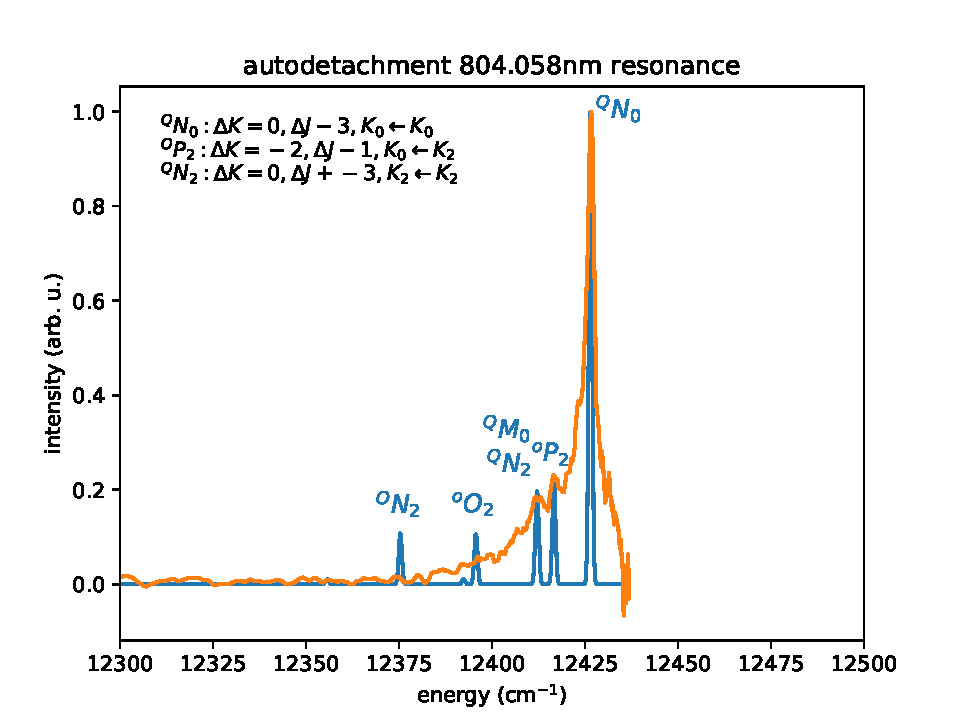
\includegraphics[width=0.5\textwidth]{scripts/804}
	\caption{resonance at 804}
	\label{fig:804}
\end{figure}

Consequently, the strongest allowed autodetachment pathway may be assigned to the $^PR_1$ absorption and $^QN_0$ autodetachment transitions,
\begin{align*}
	A^-(J = 23, K=1) \xrightarrow{^PR_1} DBS^-(J=24,K=0) \xrightarrow{^QN_0} N(J=21, K=0).
\end{align*}
Similarly, the next strongest band may be assigned to the $^RP_1$ absorption and $^OP_2$ autodetachment transitions,
\begin{align*}
	A^-(J = 33, K=1) \xrightarrow{^RP_1} DBS^-(J=32,K=2) \xrightarrow{^OP_2} N(J=31, K=0).
\end{align*}
These transitions are illustrated in the energy level diagram in Fig.~\ref{fig:804}. This result highlights how careful choice of the detachment wavelength allows one to probe specific rotational lines, and examine the rotational autodetachment mechanisms for different $\Delta J$ and $\Delta K$ transitions. Furthermore, at 804.057~nm direct detachment is only accessible from rotationally hot J/K levels in the anion, providing only a small background to the resonant transitions.

\subsubsection{Excitation pathways}
All of the experiments presented in this study so far have utilised velocity map imaging to obtain high resolution in the electron kinetic energy domain. This provides a direct measurement of the autodetachment pathways from DBS to neutral. Conversely, information about the first step, excitation of the anion up into the DBS, has been obtained indirectly from comparisons between successive measurements. 

To create a complete picture of the DBS spectroscopy, the HR-PEI spectrometer was reconfigured to run in an `electron counting' mode. This provides a direct measurement of the absorption pathways from anion to DBS. Instead of measuring the energy of each detached electron, the number of photoelectrons per laser shot was recorded while the detachment laser was scanned over the origin band. Resonances in the total photoelectron cross section reveal the excitation pathways from anion to DBS with much higher resolution. The detachment laser was scanned from 798 to 811~nm, with the resulting spectrum presented in Fig.~\ref{fig:scan}.

\begin{figure}
	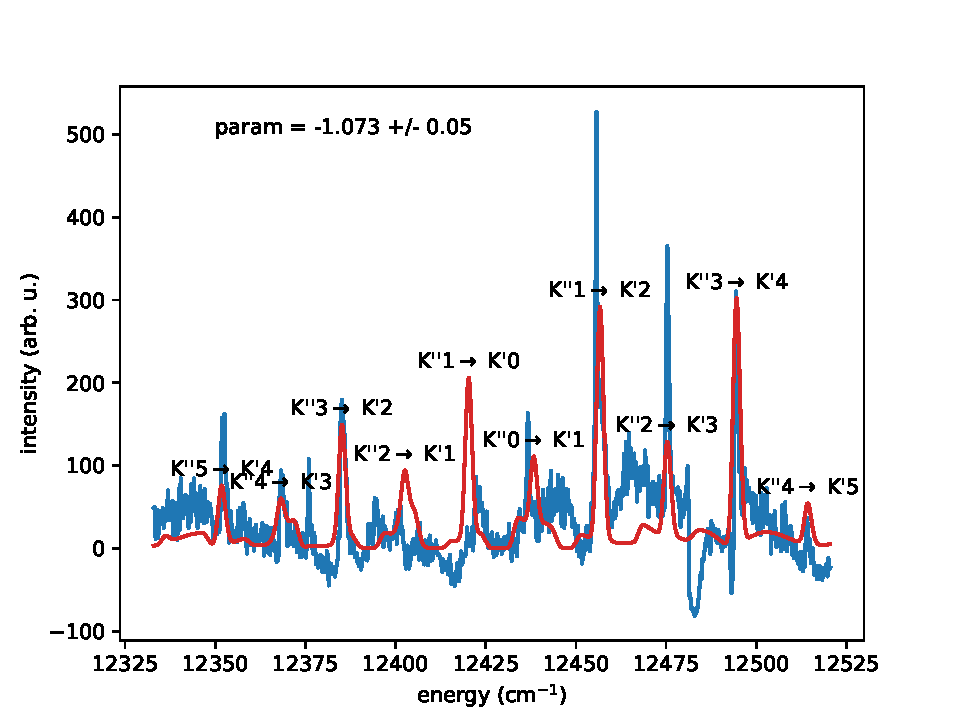
\includegraphics[width=0.5\textwidth]{scripts/scan}
	\caption{total photoelectron cross section}
	\label{fig:scan}
\end{figure}

Each sharp peak resolved in Fig.~\ref{fig:scan} may be assigned to a different $\Delta K=\pm1$ transitions from the anion up into the DBS. By fitting the full DBS rotational model constructed in this work to the experimental spectrum, the true band origin of each $K$ band may be accurately determined. This finds the origin to be centred at 12468XXX~cm$^{-1}$, representing the term energy for the anion ground state $\rightarrow$ DBS transition. The difference between the EA (xxx~cm$^{-1}$) from Fig.~\ref{fig:781} and the term energy 12468XXX~cm$^{-1}$ provides a value for the strength of the DBS binding energy of 39XX~cm$^{-1}$. Similarly to the spectra in Figs.~\ref{fig:801} and~\ref{fig:804}, excitation to the lowest rotational levels ($E_{\text{rot}}(J,K) < DBS$) will be missing from the experimental spectrum as only autodetaching transitions are recorded. 

\subsection{Implications for the DIB}
The diffuse interstellar bands (DIB) are a series of over 500 absorption lines that have been observed in the near IR and visible regions of the spectrum of the interstellar medium (ISM). While identifying the origins of these bands has been one of the major goals of astronomical spectroscopy, at the time of publication the only confirmed carrier of a DIB was C$_{60}^+$. Historically, the role of anions in the ISM has received minimal attention, as it is expected anions would be rapidly photoionised in the interstellar UV field. However, if the rate of radiative electron detachment is high relative to the rate of photodetachment, observable abundances of anions may form. Chemical models in the environment of some carbon rich stars have predicted observable abundances of $C_n^-$, $C_nH^-$ and C$_nN^-$ ions, while microwave signatures of the anion C$_6H^-$ in space have been detected experimentally, confirming that anions do play a role in some interstellar environments.

Consequently, as most anion EAs are in the visible region of the spectrum, multiple studies have suggested anion DBS transitions could be promising candidates for potential DIB carriers. This idea has been helped by the observation that the DBS in H$_2$CCN$^-$ is a potential origin of the DIB at 803.7~nm. Comparisons between astronomical observations and previous laboratory studies of H$_2$CCN$^-$ do show good agreement. However, these comparisons rely on modelling to account for the different environments between the lab studies and the ISM. Significantly, the temperature of the ISM $\sim2.7~$K is far colder than the anion temperature in the laboratory experiments.

This hypothesis may be revisited, using the complete spectroscopic model of the H$_2$CCN$^-$ DBS constructed in this work. The simulated absorption spectrum of H$_2$CCN$^-$ at 2.7K is shown in Fig.~\ref{fig:DIB} alongside the experimental spectrum at T$\sim150~$K. A composition of astronomical observations of the 803.7~nm DIB is also shown for comparison. Unlike the previous simulation, this model includes transitions to all rotational levels in the DBS, even if E$_{\text{rot}}(J,K)< $ DBS$_{BE}$.

\begin{figure}
	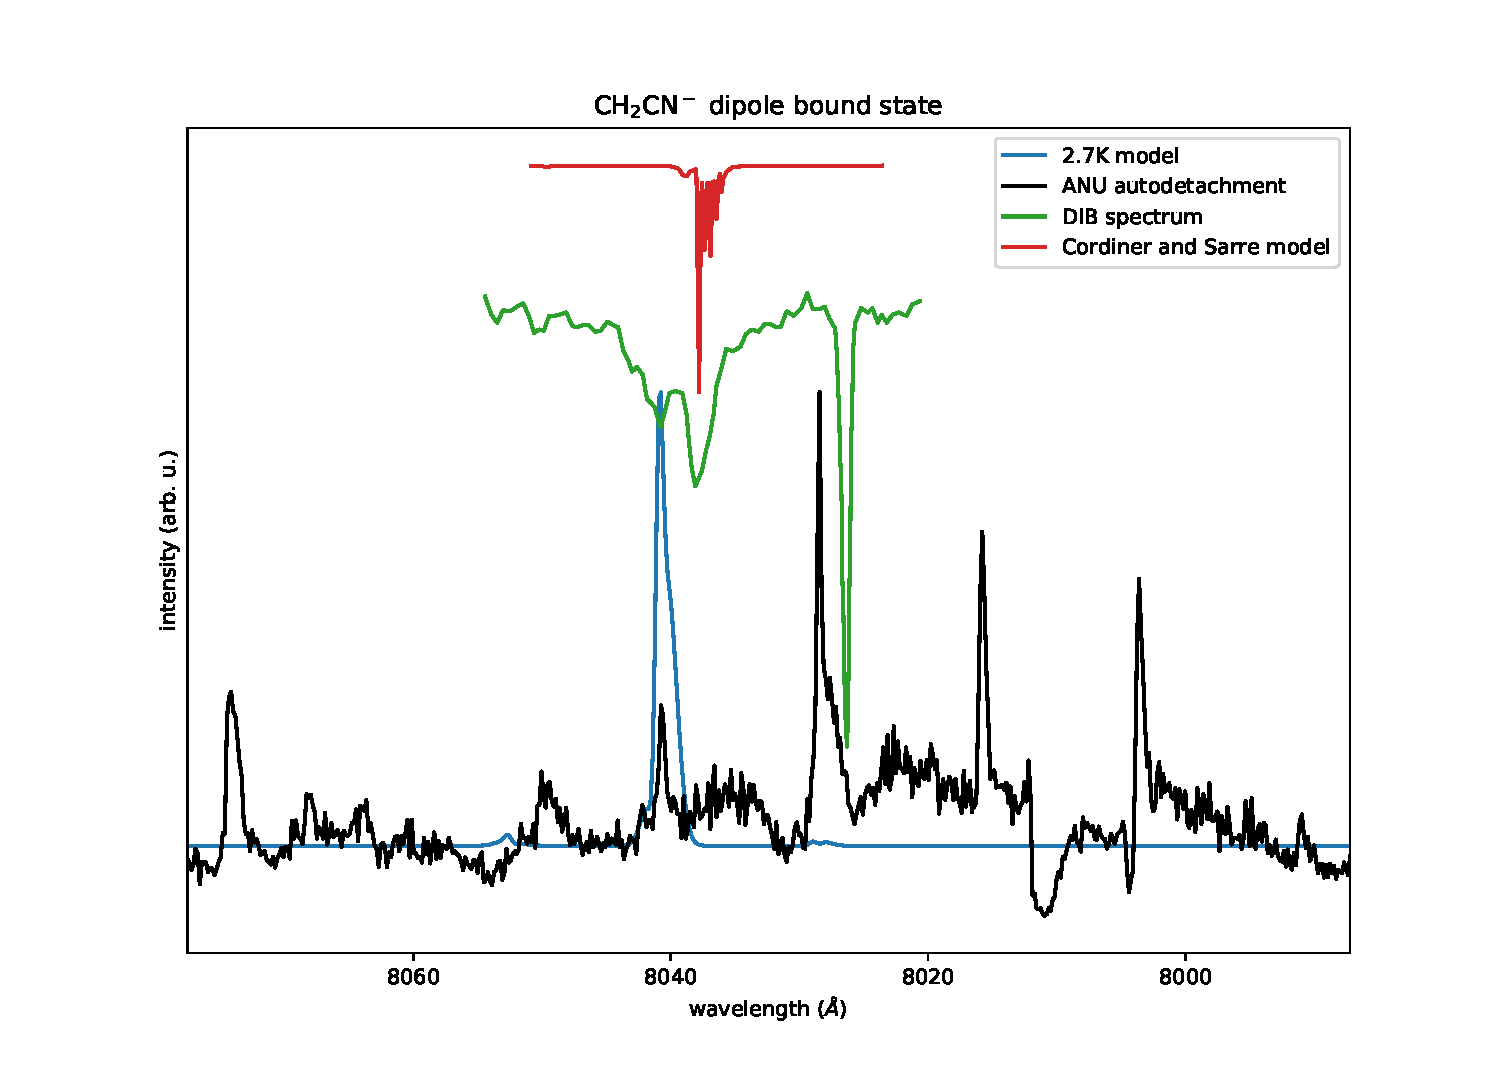
\includegraphics[width=0.5\textwidth]{scripts/DIB}
	\caption{DIB comparison}
	\label{fig:DIB}
\end{figure}

Fig.~\ref{fig:DIB} shows that the improved spectroscopic model shift the H$_2$CCN$^-$ DBS absorption spectrum by $\sim0.3$~nm. This suggests that the cyaomethylide anion is not a likley carrier of the 803.7~nm DIB, but it may be a potential carrier of the slightly weaker, nearby 804.0~nm line. However H$_2$CCN$^-$ is expected to exist in the ISM in both ortho and para forms. 





Hi~\cite{law17}

\begin{acknowledgement}
	This research was supported by the Australian Research Council Discovery
	Project Grant DP160102585.   
\end{acknowledgement}

% Create the reference section using BibTeX: 
\bibliography{May2021-H2CCN}

\end{document}
% ****** End of file apstemplate.tex ******